\documentclass[12pt,fleqn]{article}\usepackage{../common}

\begin{document}
Ders 1

Bu derste matrislerden bahsedilecek, onlarin canlanmasini, dile gelmesini
istiyoruz. Mesela alttaki gibi bir matris

\[ 
K =
\left[\begin{array}{rrrr}
2 & -1 & 0 & 0\\
-1 & 2 & -1 & 0\\
0 & -1 & 2 & -1\\
0 & 0 & -1 & 2
\end{array}\right]
 \]

nedir? Nereden gelir? Bu matris bir seyi temsil edecek, bilimsel bir
problemi cozmemizi saglayacak. 

Matrisin ozelliklerine bakalim. Ilk bakista bunun simetrik bir matris
oldugunu goruyoruz. Yani $K = K^T$. Bu tur matrisler ozellikle dengedeki
sistemler (equilibrium) problemlerinde cok ortaya cikiyorlar. Baska
ozellikler? $K$'yi buyutseydik, seyrek (sparse) olacakti, yani icinde cok
fazla sayida sifir olacakti. Su haliyle tam seyrek denemez, ama ayni
kalipla buyutulursek seyrek olur. Eger Python kullanarak sifir olmayan
elemanlari saydirmak isteseydik, sonuc ne gelecekti? 4x4 olan $K$ icin
alttaki kod su sonucu verir,

\begin{minted}{python}
K = np.array([[2,-1,0,0],[-1,2,-1,0],
              [0,-1,2,-1],[0,0,-1,2]])
print np.count_nonzero(K)
\end{minted}

\begin{verbatim}
10
\end{verbatim}

4x4 = 16 icinden 10 eleman sifir degildir. Eger 100x100 olsaydi? Matris
ayni kalibi takip ederse, yani caprazi, ve caprazin bir alti ve bir ustu
dolu kalirsa, caprazda 100 eleman olur (boyutla ayni), alt ve ustunde birer
az eleman olur, yani 99+99 = 198. Toplayalim, 100 + 198 = 298. Yani 100x100
= 10000 eleman icinden 298 eleman sifir degildir, geri kalan bir suru
eleman sifirdir. Matris seyrektir.

Numerik hesaplamada yogun (dense -sifiri fazla olmayan-) matrisler, buyuk
boyutlarda basimizi agritabilir. Seyrek matrisleri daha hizli cozmenin
yontemleri vardir, ama 1 milyon x 1 milyon bir yogun matris cozmesi
imkansiz hale gelebilir. 

Baska ozellikler? Matris uclu kosegen (tridiagonal) [1]. Bu tur matrisler cok
onemlidir, Newton sagolsun, ikinci seviye diferansiyel denklemlerden
surekli ortaya cikarlar mesela. 

Dahasi? Bu bir Toeplitz matrisi, caprazdaki degerler sabit degerler, capraz
boyunca hic degismiyorlar. Bu matrislere lineer zamana gore degismeyen
filtreler (linear time invariant filters) ismi de veriliyor, cunku her
satir birbirinin ayni (ve hesabimizda satirlarin zamani temsil ettigi
kabulunden hareketle). Python ile bir Toeplitz yaratmanin yontemi soyle:

\begin{minted}{python}
import scipy.linalg as lin
K = lin.toeplitz([2, -1, 0, 0])
print K
\end{minted}

\begin{verbatim}
[[ 2 -1  0  0]
 [-1  2 -1  0]
 [ 0 -1  2 -1]
 [ 0  0 -1  2]]
\end{verbatim}

100x100 icin Toeplitz komutuna verdigimiz tek satirda daha fazla sifir
gerekli. Icinde tamamen sifir olan bir vektor yaratiriz, basindaki birkac
elemani istedigimiz degerle atariz. 

\begin{minted}{python}
import scipy.linalg as lin
vec = np.zeros((1,100))
vec[0,0] = 2
vec[0,1] = -1
print lin.toeplitz(vec)
\end{minted}

\begin{verbatim}
[[ 2. -1.  0. ...,  0.  0.  0.]
 [-1.  2. -1. ...,  0.  0.  0.]
 [ 0. -1.  2. ...,  0.  0.  0.]
 ..., 
 [ 0.  0.  0. ...,  2. -1.  0.]
 [ 0.  0.  0. ..., -1.  2. -1.]
 [ 0.  0.  0. ...,  0. -1.  2.]]
\end{verbatim}

Seyrek matrislerle islem yaptigimizi Python'a bir sekilde belirtmemiz
lazim, eger mevcut haliyle bu matrisi cozmeye ugrasirsak, Python sifirlara
gelene kadar onlarin sifir oldugunu bilemeyecektir. 

\begin{minted}{python}
import scipy.sparse as sparse
import numpy as np
import scipy.linalg as lin
vec = np.zeros((1,100))
vec[0,0] = 2
vec[0,1] = -1
K = lin.toeplitz(vec)
A = sparse.lil_matrix(K)
print A.shape
\end{minted}

\begin{verbatim}
(100, 100)
\end{verbatim}

Yanliz yukarida yogun matrisi once yarattim, sonra onu degistirerek seyrek
matris yarattim, daha iyisi bastan bir seyrek matris yaratmakti. Neyse, bu
yontemi ileri de gorecegiz. 

Daha derine inelim simdi. $K$ matrisi tersi alinabilen (invertible) bir
matris midir? Evet. Bu ne demektir? $KK^{-1} = I$, ve $I$ matrisi birim
(identity) matrisidir, Python'da \verb!np.eye(N)! komutuyla 
yaratilabilir. 

Bir matrisin tersinin alinip alinamayacagini nasil anlayabiliriz? Bu cok
onemli, temel bir sorudur. 

Bazilarinin aklina determinanti hesaplamak gelebilir. Fakat hocanin ilk
secimi bu degil. Onun tercihi satir indirgemek (row reduce). Tavsiyesi bu,
onunuzde bir matris var, ve icinde neler olup bittigini
bilmiyorsunuz. Satir indirgeyin. 

Bu nasil yapilir? $K$'in caprazinin altindaki -1 degerlerini sifirlamak
istiyorum. Orayi temizlemek istiyorum, cunku matrislerim eger ucgensel
(triangular) ise, olan biteni aninda gorebilirim.

Birinci satiri ikiye bolup, ikinci satira eklerim. Terminoloji: 0,0
kordinati (en ust sol kose) bu islem sirasinda pivot oldu. 

\begin{verbatim}
 [ 2 -1    0  0]
 [ 0  3/2 -1  0]
 [ 0 -1    2 -1]
 [ 0  0   -1  2]
\end{verbatim} 

Simdi pivot 3/2, ve onun altindaki degeri temizlemek istiyoruz. Ikinci
satirin 2/3'unu alta eklersek, oradaki -1 sifirlanir. 

\begin{verbatim}
 [ 2 -1    0    0]
 [ 0  3/2 -1    0]
 [ 0  0    4/3 -1]
 [ 0  0   -1    2]
\end{verbatim}

ve sonunda

\begin{verbatim}
 [ 2 -1    0      0]
 [ 0  3/2 -1      0]
 [ 0  0    4/3   -1]
 [ 0  0    0    5/4]
\end{verbatim}

Bu gercekten hizli bir islem oldu. Python da determinanti zaten boyle
bulacakti. Yoketme (elimination) kullanacakti, teker teker -1'leri
yokedecekti. Peki determinantin degeri nedir? 5. Niye 5? Cunku elimizdeki
artik ucgensel bir matris, ve boyle matrislerde caprazdaki elemanlari
birbiriyle carpmakla determinant hemen hesaplanir. Python aynen boyle
yapacakti, $2 \cdot 3/2 \cdot 4/3 \cdot 5/4 = 5$.

Simdi tersinin olup olmadigi sorusuna geri donelim: Bir ust ucgensel (upper
triangular) matris ne zaman tersine cevirilebilir haldedir? Determinant
kelimesini kullanmamiza gerek yok, capraza bakariz, eger bu capraz sifir
degeri olmayan bir capraz ise bu matris tersine cevirilebilir
demektir. Terminoloji: demek ki elimizde N tane ($K_4$ icin 4) tane sifir
olmayan pivot var. 

1. dersin amaclarindan biri matrislere isim vermek. $K$ matrisi bunlardan
biri, onemli bir matris, onu ileride tekrar gorecegiz, gorunce
taniyacagiz. 

\[ 
C = 
\left[\begin{array}{rrrr}
2 & -1 & 0 & -1\\
-1 & 2 & -1 & 0\\
0 & -1 & 2 & -1\\
-1 & 0 & -1 & 2\\
\end{array}\right]
\]

Peki su matris? Toeplitz formunda ama ust sag ve alt sol koselerde ekstra
bir -1 degeri var. Fakat iddia ediyorum ki bu matris tersine cevirebilir
degil ve bunun icin determinant, ya da yoketme teknigine gerek
yok. Terminoloji: Matrise $C$ denilmesi onun degerlerinin dairesel
(circulant) olmasindan ileri geliyor. -1 degerlerine bakin, sanki bir
yuvarlak olusturuyorlar, sifir degerleri ayni sekilde. 

Devam edelim: Diyelim ki $C$ bir vektoru carpiyor (zaten matrislerin tek
amaci bu, vektorler ile carpilmak), ve ortaya sifir vektoru cikiyor. Bos
olan vektor ne olabilir?

\[ C = 
\left[\begin{array}{rrrr}
2 & -1 & 0 & -1\\
-1 & 2 & -1 & 0\\
0 & -1 & 2 & -1\\
-1 & 0 & -1 & 2\\
\end{array}\right]
\left[\begin{array}{r}
\\
\\
\\
\\
\end{array}\right]
=
\left[\begin{array}{r}
0\\
0\\
0\\
0
\end{array}\right]
 \]

Su olabilir

\[ C = 
\left[\begin{array}{rrrr}
2 & -1 & 0 & -1\\
-1 & 2 & -1 & 0\\
0 & -1 & 2 & -1\\
-1 & 0 & -1 & 2\\
\end{array}\right]
\left[\begin{array}{r}
1\\
1\\
1\\
1\\
\end{array}\right]
=
\left[\begin{array}{r}
0\\
0\\
0\\
0
\end{array}\right]
 \]

Iddia ediyorum ki boyle bir vektorun olabilmesi $C$'nin tersine
cevirilebilir olma olasiligini yoketti. Nasil? 

Eger $C$'nin tersi olabilseydi, $Cu = 0$ denklemi ne olurdu? Iki tarafi bu
``olabilen'' $C^{-1}$ ile carpip sonuca bakalim:

\[ C^{-1}Cu = C^{-1}0 \]

\[ I u = 0 \]

\[ u = 0 \]

Yani eger $C$'nin tersi olsaydi, $Cu = 0$ denkleminin tek sonucu $u=0$
olurdu. Fakat bu boyle degildir, ustte icinde 1 olan vektor bunun kaniti. O
zaman bir uyusmazlik, absurtluk elde ettik, demek ki $C$'nin tersi oldugu
iddiasi yanlistir.

Fiziksel olarak $K$ ve $C$'nin kutle ve yay sistemi olarak kabul
edebiliriz. Mesela $K$ soyle bir sistemi temsil edebilir:

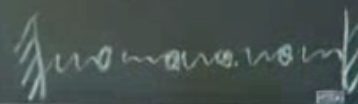
\includegraphics[height=1cm]{1_5.png}

Yuvarlak olan $C$ sistemi sunu temsil edebilir

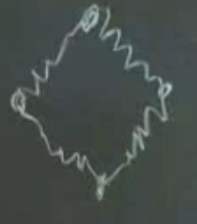
\includegraphics[height=2cm]{1_6.png}

Resimdeki noktalar kutleler, ve yaylar o kutleleri birbirine bagliyorlar.

$T$ Matrisi

Bu matris $K$'ye benzer, fakat en ust satirda 2 yerine 1 var. 

\[ 
\left[\begin{array}{rrrr}
1 & -1 & 0 & 0\\
-1 & 2 & -1 & 0\\
0 & -1 & 2 & -1\\
0 & 0 & -1 & 2
\end{array}\right]
\]

Kutle ve yay sistemine donersek bu matris bir ucu serbest olan bir mekanik
sistemi gosterebilir. 

B Matrisi

\[ 
\left[\begin{array}{rrrr}
1 & -1 & 0 & 0\\
-1 & 2 & -1 & 0\\
0 & -1 & 2 & -1\\
0 & 0 & -1 & 1
\end{array}\right]
\]

Bu sistem de her iki ucu da serbest olan bir sistemdir. Bu sistemi alip
istedigimiz yere goturebiliriz. 

Son iki matrisin ikisi de simetriktir, ucgensel ve kosegen (diagonal)
matrislerdir. Niye ucgensel ve kosegen? Cunku her kutle sag ve solunda
tek bir (diger) kutleye baglidir, o yuzden bagli olmadigi kutlelere olan
matris degeri 0 olarak gosterilir, bu da bir ucgensel kosegen sistem
ortaya cikarir.

Ama T ve B artik Toeplitz degildir. 

Bu noktada s�n�r sartlari (boundary conditions) kavramina vurgu yapmakta
yarar var. Mekanik sistemde ucun ne oldugu matrislere s�n�r sarti olarak
yansiyor. Ve bu sartlar bir sistemin cozulmesinde son derece onemli. Hoca
kendisine bir problemle gelenlere genelde ilk once bu soruyu soruyor o
yuzden: ``s�n�r sartlarin ne?''. 

Tersine cevirilme durumu? T tersine cevirilebilir, B cevirilemez. B icin
yine ayni u = [1 1 1 1] ispatini kullanabiliriz. 

K, T, B, C matrislerini ayni anda yaratan bir Python programi
surada. Kullanim mesela 4x4 boyutlari icin \lstinline!K, T, B, C = ktbc(4)!
seklinde, bu bize tum ozel matrisleri bir kerede olusturuyor.

\begin{minted}{python}
import scipy.linalg as lin

def ktbc(n):
    vec = np.zeros((1,n))
    vec[0,0] = 2
    vec[0,1] = -1
    K = lin.toeplitz(vec)
    T = np.copy(K)
    T[0,0] = 1
    B = np.copy(K)
    B[0,0] = 1
    B[n-1,n-1] = 1
    C = np.copy(K)
    C[n-1,n-1] = 1
    
    return K, T, B, C
\end{minted}

Kapatirken su ozellikleri de ekleyelim. 

K, T pozitif kesin (positive definite) matrislerdir. 

C, B pozitif yari-kesin (positive semi-definite) matrislerdir. 

Eger simetrik bir matrisim var ise ve pivotlarin hepsi pozitif ise, o
matris hem tersine cevirelebilir, hem de pozitif kesin demektir. Yani bir
matrise bakariz, yoketme teknigini uygulariz sonra pivotlarina bakariz. 

Pozitif kesinlik cok onemli bir kavramdir, lineer cebirin tamamini biraraya
getirir sanki, ozdegerlere (eigenvalue) baglidir, least square yontemine
baglidir, determinantlar. Her yerden cikar. 

Geriye Dogru Farklilik Matrisi

Python \verb!toeplitz! cagrisinin degisik bir sekilde kullanarak geriye
dogru farklilik (backward difference) matrisi de yaratabiliriz. Bu
kullanimda matrisin sol kolonunu, ve ust satirini tamamen belirtmek
gerekiyor.

\begin{minted}{python}
import scipy.linalg as lin

D = lin.toeplitz([1, -1, 0, 0], [1, 0, 0, 0])
print D
\end{minted}

\begin{verbatim}
[[ 1  0  0  0]
 [-1  1  0  0]
 [ 0 -1  1  0]
 [ 0  0 -1  1]]
\end{verbatim}

Cozulmus Soru 1.1 B

Soru: $T$ matrisini $H$ matrisine cevir bunu $J$ matrisini kullanarak
yap. 

\[ H = 
\left[\begin{array}{rrr}
2 & -1 &  0\\
-1 & 2 & -1\\
0 & -1 & 1
\end{array}\right]
 \]

\[ T = 
\left[\begin{array}{rrr}
1 & -1 &  0\\
-1 & 2 & -1\\
0 & -1 & 2
\end{array}\right]
 \]

Kitaptaki bu sorunun cozumundeki $J$ matrisi birimsel matrisin tersidir, 
su sekildedir:

\[ 
\left[\begin{array}{rrr}
0 & 0 & 1\\
0 & 1 & 0\\
1 & 0 & 0
\end{array}\right]
 \]

Yani 1 sayilari sola yatik caprazda degil saga yatik caprazda. Bu matrisin
carpim islemi sirasinda ilginc etkileri var. Eger sagdan carpilirsa bir
matrisin her satirinin icindeki sirayi tersine ceviriyor. Eger soldan
carpilirsa her kolon icindeki sirayi tersine ceviriyor. $J*T*J$ carpimi
aradigimiz sonuc. Yani satirlari cevirdikten sonra, kolonlari cevirince
istedigimiz sonuca erisiyoruz. Python kodlari

\begin{minted}{python}
import scipy.linalg as lin
T = lin.toeplitz([2, -1, 0])
T[0,0] = 1
J = np.fliplr(np.eye(3))
print T
print np.dot(T,J)
print np.dot(J, np.dot(T,J))
\end{minted}

\begin{verbatim}
[[ 1 -1  0]
 [-1  2 -1]
 [ 0 -1  2]]
[[ 0. -1.  1.]
 [-1.  2. -1.]
 [ 2. -1.  0.]]
[[ 2. -1.  0.]
 [-1.  2. -1.]
 [ 0. -1.  1.]]
\end{verbatim}

Soru 1.1 2

\begin{minted}{python}
import scipy.linalg as lin

T = lin.toeplitz([2, -1, 0])

T[0,0] = 1

U = np.array([[1, -1, 0],
              [0, 1, -1],
              [0, 0, 1]])

print np.dot(U.T,U)
print np.dot(U,lin.inv(U))
print np.dot(lin.inv(U), lin.inv(U).T)
\end{minted}

\begin{verbatim}
[[ 1 -1  0]
 [-1  2 -1]
 [ 0 -1  2]]
[[ 1.  0.  0.]
 [ 0.  1.  0.]
 [ 0.  0.  1.]]
[[ 3.  2.  1.]
 [ 2.  2.  1.]
 [ 1.  1.  1.]]
\end{verbatim}

Soru 1.1.5

\begin{minted}{python}
import scipy.linalg as lin

K, T, B, C = ktbc(3)
print lin.inv(K)
print lin.det(K)
print lin.det(K) * lin.inv(K)

K, T, B, C = ktbc(5)
print lin.det(K)
print lin.inv(K)
print lin.det(K) * lin.inv(K)
\end{minted}

\begin{verbatim}
[[ 0.75  0.5   0.25]
 [ 0.5   1.    0.5 ]
 [ 0.25  0.5   0.75]]
4.0
[[ 3.  2.  1.]
 [ 2.  4.  2.]
 [ 1.  2.  3.]]
6.0
[[ 0.83333333  0.66666667  0.5         0.33333333  0.16666667]
 [ 0.66666667  1.33333333  1.          0.66666667  0.33333333]
 [ 0.5         1.          1.5         1.          0.5       ]
 [ 0.33333333  0.66666667  1.          1.33333333  0.66666667]
 [ 0.16666667  0.33333333  0.5         0.66666667  0.83333333]]
[[ 5.  4.  3.  2.  1.]
 [ 4.  8.  6.  4.  2.]
 [ 3.  6.  9.  6.  3.]
 [ 2.  4.  6.  8.  4.]
 [ 1.  2.  3.  4.  5.]]
\end{verbatim}

Soru 1.1.22

Cozulmesi istenen denklem $du^2/dx^2 = 1$, elastik cubuk problemi ve
cubugun iki tarafi sabitlenmis.

\begin{minted}{python}
import scipy.sparse as sparse
import scipy.sparse.linalg
import scipy.linalg as lin

n = 1000
vec = np.zeros((1,n))
vec[0,0] = 2; vec[0,1] = -1
K = lin.toeplitz(vec)
A = sparse.csc_matrix(K)
e = np.ones((n,1))

u = sparse.linalg.spsolve(A,e)
plt.plot(u)
plt.savefig('1-1-22.png')
\end{minted}

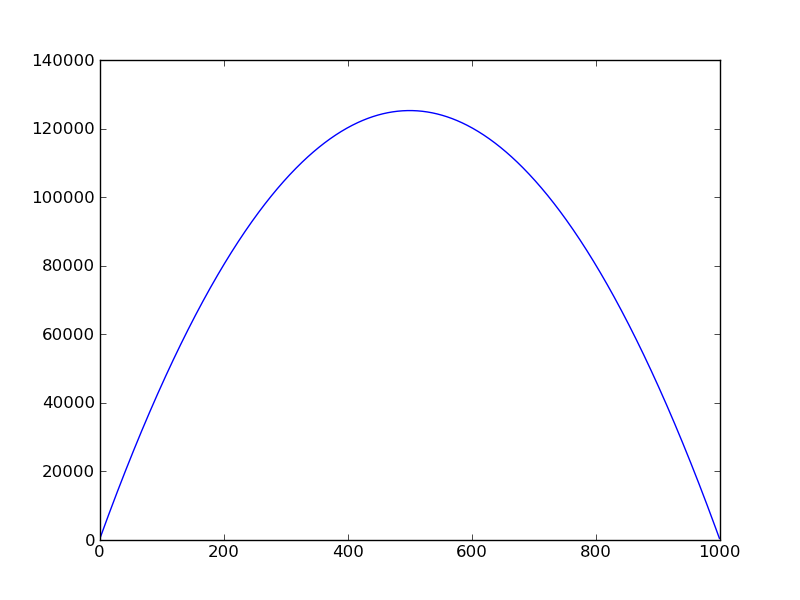
\includegraphics[height=5cm]{1-1-22.png}

Sonuc ustteki grafik gibi olmali. Yani cozumumuz olan $u$ degerleri bir
parabol olusturuyorlar. Bu demektir ki cubugun orta noktalari daha fazla
yer degistiriyor, uc noktalari daha az yer degistiriyor. 

Elastik Cubuk

Derste cokca kullanilan elastik cubuk kavramindan simdi bahsetmek iyi
olur. Bu cubuk tek boyutlu ve sadece boyuna dogru (yana dogru degil) uzayip
kisalabilen matematiksel bir kurgu. Bu cubugu hayalimizde birbirine
zincirler ile bagli sonsuz sayida ufak parcacigin toplami olarak
dusunebiliriz. $x$ ve $u(x)$ baglaminda ise cubugun iki kere fotografinin
cekildigini dusunelim. Ilk fotografta $x$ bu cubugun uzerindeki bir
parcacik. $u(x)$ ise tum agirliklar, kuvvetler etkilerini gosterip uzama,
kisalma bitince cekilen {\em ikinci} fotografta ilk resimdeki $x$
noktasinin ne kadar yer degistirmis oldugu.

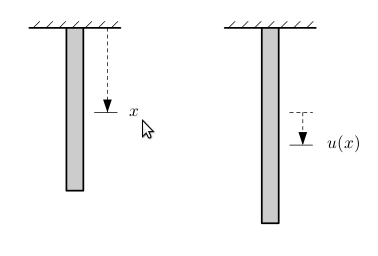
\includegraphics[height=4cm]{1_7.png}

``Ucu sabitlemek'' gibi kavramlar duyacagiz, bunlar bazen fiziksel olarak
anlamli, bazen ise ikinci fotografta esneme sonrasi hangi noktaya
gelindiginin onceden belirlenmesi anlaminda. $du/dx$ gibi bir turevi
irdelerken ise ortada zaman olmadigini dikkate alalim, turev $x$'e gore
yani ilk resimdeki parcacigin yeri. O zaman $du/dx$ ikinci resimdeki
esnemenin cubuktaki yer arttikca (asagi indikce) ne kadar degistigi. 

Denklemin saginda yer alan degerler, sisteme disaridan verilen guc olarak
gorulebiliyor, hakikaten de degisimin ikinci turevi ivmedir. 1.2.22
sorusunu gorsel olarak nasil hayal edebiliriz? Cubugun iki ucu sabitlenmis,
o sebeple K matrisi kullaniyoruz zaten, boylece sinir sartlari dahil oluyor.

Python, VPython uzerinden kullanilabilecek KineticsKit adli paket sistemi
zihinde canlandirmak icin yardimci olabilir. Birbirine esit uzaklikta, ayni
kutlede ve arasinda yaylar olan 7 tane topu birakinca ne oldugunu simule
edebiliriz. Resimdeki sol kisim baslamadan once, sag kisim yercekimi isini
bitirdikten ve toplar durduktan sonrasini gosteriyor.

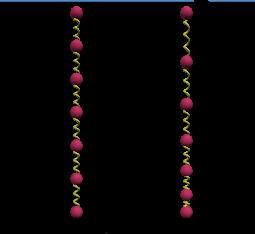
\includegraphics[height=5cm]{elastic_uniform_load.png}

Alttaki program hem gorsel simulasyonu yapacak, hem de toplarin once ve
sonra degerlerini hatirlayarak yercekimi sonrasi aradaki farki
hesaplayacak. Sonuclara bakinca hakikaten de ortadaki toplarin daha fazla
hareket ettigini gorebiliyoruz. Grafiksel olarak dusunursek te mantikli,
uste yakin toplar ustten bagli olduklari icin fazla uzaklasamiyorlar,
ortalara yakin toplar, bir ustlerinden de aldiklari ek mesafe sayesinde
daha fazla yer degistirebiliyor. Ama alt kisima yaklastikca orada bir
birikme oluyor, cunku alt uc kisim da sabitlenmis. 

\inputminted{python}{elastic_uniform_load.py}

Ekler

[1] Uclu kosegenlik, matris caprazi, onun bir ustu ve alti haricindeki tum
diger elemanlarin sifir oldugu bir matristir. 

\end{document}
